% !TeX root = ../main.tex
% Add the above to each chapter to make compiling the PDF easier in some editors.

\chapter{Methodology}\label{chapter:methodology}

\section{Terminology}
\label{sec:terminology}

Before we dive into technical explanations, we want to clear some potential terminology confusion.

In the original DICE release from Microsoft \cite{England2016}, the identifier of a component is called the Firmware ID (FWID).
The TCG consortium later renamed it TCB Component Identifier (TCI).
We believe this is to emphasize that the TCI does not necessarily have to be the hash of a firmware binary, but could also be, for example, the embedded ID of a hardware component.
However, TCG has not fully implemented this terminology renaming.
Their DICE Attestation Architecture \cite{TCGAttestation2021} defines an X.509 extension that contains the TCIs.
They continue to be referred to as FWIDs in the formal definition of this extension, while everywhere else they are referred to as TCIs.
In personal correspondence with TCG, we have learned that this is due to backwards compatibility.
The old term FWID is retained whenever it is used in something that is alive in the long term, like formal definitions, and the new term TCI in assets that can be updated more quickly, such as the specification text.
Therefore, we will use the term TCI in this theoretical chapter, and in the implementation chapter (\autoref{chapter:implementation}) we will use the term FWID, just as it is common practice at the TCG.

% Prover/Verifier (in many earlier papers) vs. Attester/Verifier/Relying Party (RFC)


\section{Architectural overview}

\begin{figure}[htpb]
  \centering
  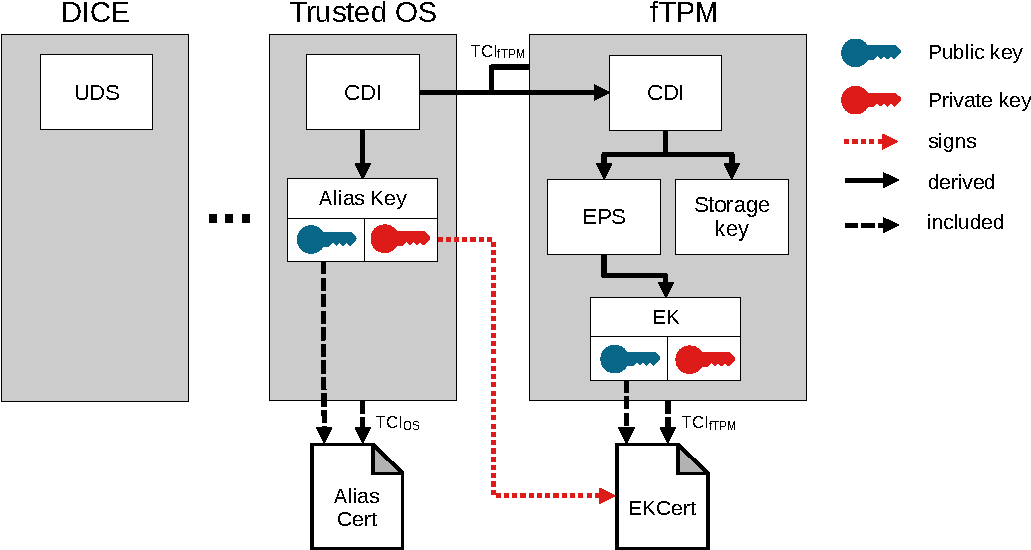
\includegraphics[width=1\linewidth]{figures/architecture.pdf}
  \caption{The architecture of our system.} \label{fig:architecture}
\end{figure}


The architecture of our proposed and later implemented system is illustrated in \autoref{fig:architecture}.
As you might notice, it is similar to our overview picture of DICE (\autoref{fig:dice-layers}).
This is to be expected, since our system uses DICE.
We leverage the DICE as our static root of trust for measurements (S-RTM).
Static in this context means that it uses the trusted state that a device has at the always same point in time, here after switching on, for further measurements.
This is in contrast to a dynamic RTM (D-RTM), which is able to do this at any time, e.g., Intel SGX.

The boot process continues from here in the usual DICE manner until the firmware TPM is reached.
The component that measures the fTPM is usually the trusted operating system running in EL1 in the secure world, as seen in \autoref{fig:arm_trustzone_arch}.
Like any other DICE component, the fTPM receives its secret Compound Device Identifier (CDI) from its predecessor layer.
Recall that the CDI is tied to the identity of the fTPM including the entire underlying firmware stack and the UDS.
Two values are derived from the CDI.

% Storage Key generation

First, the storage key is generated.
This is a symmetric encryption key that is used to encrypt the fTPM storage space in RAM before it is written to a persistent storage space such as a hard disk drive (HDD).
At no time does the HDD see plain text data (\autoref{fig:storage-encryption}).
Since the storage key is derived from the CDI, the old storage data is inaccessible if the identity of the TPM changes, e.g., due to a TPM modification or an update of a previous firmware component, which is equivalent to a full manufacturer reset.
This enables the property that an fTPM storage must never be accessible to another TPM.

\begin{figure}[htpb]
  \centering
  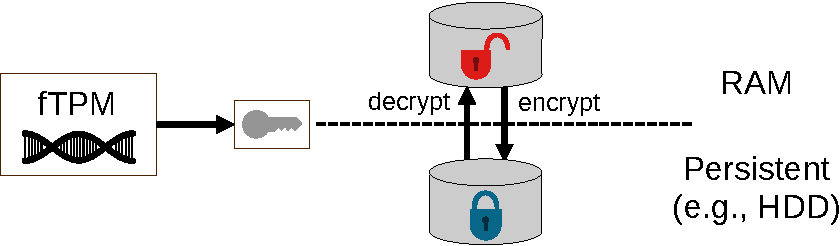
\includegraphics[width=0.8\linewidth]{figures/storage-encryption.pdf}
  \caption{The fTPMs' storage is protected by a key derived from its identity.} \label{fig:storage-encryption}
\end{figure}


% EPS Generation

Then, the primary endorsement seed (EPS) is generated.
It is the seed that is used to generate the primary endorsement key (EK).
A primary key in the sense of the TPM means that it has no parent key, but a parent seed, here the EPS.
The indirection of generating the CDI via the EPS instead of generating the EK directly from the CDI is introduced because the code of fTPMs can be hardcoded to use the EPS during EK generation.
And we want our system to require as few modifications to TPM code as possible.

% Device identification

The EK of a dedicated TPM represents the long-term identity of the device as long as the TPM is not soldered away.
Our EK does not do this because a firmware TPM is software-based and changes every time the fTPM or the underlying firmware is modified, without the host device changing.
Instead, we use the DICE for this, which is hardware-based.
Its DeviceID key, as the name suggests, represents the device identity.
Note that the DeviceID contains the identity of layer 0 of the boot chain, i.e., the first mutable code.
This can also be seen in \autoref{eq:dice_deviceID}.
For this reason, the DICE specification suggests keeping the first mutable code as small as possible so that it remains constant throughout the life of the device \cite{dice-layering-arch}.

% EK is a signing key

By default, the EK is a restricted encryption key.
It is not used for signing because the resulting signatures may reveal the TPMs' identity.
Therefore, the usual procedure is to create a short-lived attestation key (AK) on the TPM.
The verifier communicates the public part of the AK to a third party privacy CA who ensures that the holder of the AK is the same as the holder of the EK.
The privacy CA then issues an attestation certificate confirming that the AK originates from a genuine TPM, without revealing the identity of the TPM.
Finally, the AK can be used by the TPM to sign attestation evidences in a private fashion.
We waive this separation and use the EK directly for attestations to avoid the need for a third party CA.

% EKCert is an AliasCert

The DICE and the TPM infrastructure intersect at the EK certificate.
From the DICE's point of view it is an alias certificate, from the TPM's point of view it is the EK certificate.

\section{The identity of a firmware TPM}

DICE offers two identities for each component.
The TCI and the CDI.
As shown in \autoref{eq:dice_cdi}, the CDI of a component changes when (i) the identity of the hardware changes, i.e., the UDS, (ii) the identity of a preceding component changes, or (iii) the component itself changes.
In contrast, the TCI is the identity of a single component, considered in isolation, usually the hash of its binary.
It only changes when the component itself is changed, regardless of the hardware or preceding components.
So, while a CDI should be statistically unique since it is derived from a UDS with this property, a given TCI can be found on many devices if they contain exactly the same software component.
Note that the TCI is part of the CDI, as shown in \autoref{fig:identities}.

\begin{figure}[htpb]
  \centering
  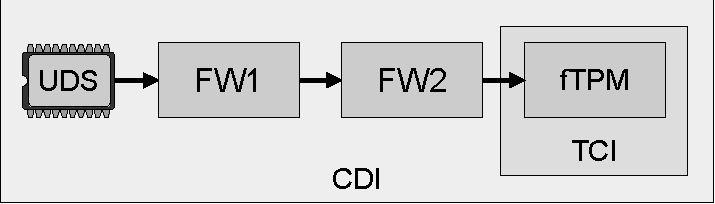
\includegraphics[width=0.6\linewidth]{figures/identities.pdf}
  \caption{Visualizing the difference between the CDI and the TCI from the perspective of an fTPM component. The identity of the hardware is provided in the form of the UDS.} \label{fig:identities}
\end{figure}


Hence, we decided to derive the identity of an fTPM, i.e., its EK, ultimately from the CDI.
This binds the identity of the fTPM to any security-relevant component preceding it.
The rationale for this is that once a previous component has changed, it is unknown whether it has gone into a benign or malicious state.
And if it is malicious, it could change the firmware TPM and thereby access its sensitive material such as private keys.
Although this is later recognized by the verifier during remote attestation, sensitive data could still be leaked.
If the identity of the firmware TPM is extended to everything prior to the fTPM, its data is no longer accessible as soon as something preceding it changes.
This is due to the derivation of the storage key from the CDI.
And this behavior should also be reflected in the EK, so that the storage key and the EK should always change together or not change at all.

% TODO: Vielleicht zu implementation
The TCI (and thus the CDI too) must also represent security-relevant configurations.
Compilation flag configurations are already inherently part of the TCI, as they are embedded in the final binary and are therefore automatically measured as part of the measurement of the binary.
Of more interest are the configurations that are not part of the binary.
They are usually provided in well-known formats such as \texttt{json} or \texttt{xml}.
However, Microsoft's fTPM reference implementation does not contain such configurations, which simplifies the TCI generation of our fTPM by limiting it to the measurement of the fTPM binary data.
The TPM's storage cannot be part of its identity as it changes during runtime after each data write, e.g., storing an arbitrary key.
This is a problem because DICE only runs during the boot time in which the identity of the fTPM is measured.
The identity of the fTPM must not change afterwards, otherwise the identity reported by DICE and the actual identity of the fTPM would be inconsistent.
We also do not want to restrict the permissible values of the working data of an fTPM.

% Depending on the point of view, there are two identities of an fTPM, as shown in \autoref{fig:identities}.
% There is the identity of the fTPM measured by DICE, which consists of the hash of the binary and the component configurations as for all DICE components, as shown in \autoref{fig:ftpm-identity}.
% This identity is referred to as the TCI.
% Compilation flags are not part of these configurations, as they are embedded in the final binary and are therefore automatically measured as part of the measurement of the binary.
% Of more interest are the configurations that are not part of the binary.
% They are usually provided in well-known formats such as \texttt{json} or \texttt{xml}.
% However, Microsoft's fTPM reference implementation does not contain such configurations, which simplifies the TCI generation of our fTPM by limiting it to the measurement of the fTPM binary data.
% The TPM's storage cannot be part of its identity as it changes during runtime after each data write, e.g., storing an arbitrary key.
% This is a problem because DICE only runs during the boot time in which the identity of the fTPM is measured.
% The identity of the fTPM must not change afterwards, otherwise the consistency of the identity transmitted by DICE and the actual identity of the fTPM would differ.
% We also do not want to restrict the permissible values of the working data of an fTPM.
% In summary, the CDI keeps being updated from layer to layer, the TCI is calculated for each layer individually.
% Then, there is also the identity of the fTPM in the TPM context, which is represented by its EK.
% This identity is not only bound to the binary and the configuration of the fTPM, but also the entire underlying firmware stack.
% We derive the EK from the TPMs CDI, which is derived of the measurements of all preceding firmware components and the TPMs' TCI, see \autoref{eq:dice_cdi}.

% \begin{figure}[htpb]
  \centering
  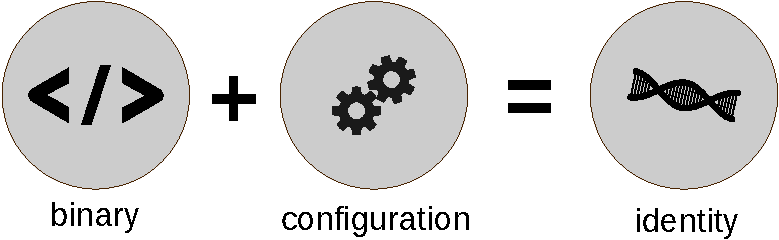
\includegraphics[width=0.6\linewidth]{figures/ftpm-identity.pdf}
  \caption{The accumulation of the binary and its configuration to its identity.} \label{fig:ftpm-identity}
\end{figure}


% Configurations required
% Does contain whole firmware stack?
% Data cannot be considered, since changes during runtime, not represented by DICE which only happens at boot-time
% What happens if identity changed? -> Data not accessible, in essence, fTPM fully reset
% https://trustedfirmware-a.readthedocs.io/en/latest/design_documents/measured_boot.html#critical-data

% \section{Provisioning process}

% To summarize, attestation key provisioning must ensure that only valid attestation key material is established in Attesters [RFC 9334]

\section{Attestation process}
\label{sec:attestation_process}

EKpriv = private portion of EK
EKpub = public portion of EK
EKcert = certificate with EKpub as subject

% Check also for revocation of manufacturer cert

% We use explicit attestation. See DICE Layering Spec 7.2
% See 8.1.1.2 for an example about implicit attestation
% Implicit attestation would require to know all resulting public keys in EKcert, which would require that we booted it up in a controlled manner beforehand and stored the resulting code.
We use an explicit attestation procedure.
This makes it sufficient for the verifier to know its trusted TCIs, whereas implicit attestation would require a database of trusted Alias public keys representing a trusted component.
And since each Alias public key is device unique, as it roots in the device's unique UDS, the verifier would need to know all Alias public keys for each component on every device he trusts, which we consider unrealistic.
Also, this would be a hindrance as the verifier should be able to establish trust into an unknown device by trusting the DICE manufacturer, and knowing the identities of trustworthy firmware.

% Secure channel must be established by requiring communication with the private key corresponding to the public key in the EKcert.
% This allows a verifier to validate that the prover is in posession of the private key, and hence, the included identities in the certificate chain are trustworthy.

\subsection{Does the verifier trust the prover's fTPM?}

It is exactly the purpose of our system to make this question answerable for the verifier.
First, the verifier needs to verify whether the signatures of the DICE certificate chain are valid, and that the root certificate from the manufacturer is considered trusted.
This also involves checking if the manufacturer certificate or the Device ID certificate was revoked.
Such an event might occur if the security of an old DICE implementation is broken, and the manufacturer wants to reflect this.
Then, the verifier can traverse the certificate chain starting from the root and verify whether each component represented by a certificate is trusted, by checking the embedded TCI.
An untrusted component must be assumed to lie about its conducted measurements.
For example, it can modify the subsequent component without reflecting this in the measurement of the TCI.
Consequently, as soon as a component is untrusted, all subsequent components have to be considered untrusted as well.
This behavior is also represented mathematically in \autoref{eq:dice_attestation}.
Therefore, trusting the fTPM requires to trust all underlying firmware components.

\begin{equation}
    \label{eq:dice_attestation}
    C_{i, \, trusted} \, \coloneqq \, \bigwedge_{k=0}^{i} trusted(C_{k})
\end{equation}

After doing this, the verifier can only state that ``I trust the certificate chain and the components of \emph{some} machine represented by it.''
This is due to the possibility of any actor to simply replay the certificate chain.
But we need to promote the \emph{some} to \emph{the machine I communicate with}.
This is solved in higher level protocols where the prover is required to be in control of the private part of the EK which corresponds to the EK of the EK certificate, e.g., this is answered as part of whether the verifier can trust the quote.
Hence, the verifier also needs to trust that the fTPM did not leak the EK private key, as this would not only allow to replay a whole certificate chain, but even succeed the higher level protocols with the leaked EK private key.
The verifier can derive whether it considers the EK private key of the fTPM as not leaked based on the fTPM's TCI value, as one requirement of trusting a TCI must be whether the verifier considers the component to keep its security guarantees.


\subsubsection{Example security policies for a component}

The $trusted$ function of \autoref{eq:dice_attestation} checks the information provided by a certificate~$C$ against security policies defined by the verifier.
In the following, we would like to present some example policies for improving comprehensibility for the reader.

\begin{itemize}
    \item We generally do not trust the component's manufacturer and therefore, do not trust the component.
    \item The component is up-to-date, and there are no known vulnerabilities and therefore, we trust the component.
    \item The component is outdated, but all updates are only functional instead of security-relevant, so we still trust it.
    \item We do not know the TCI of the component. We follow a 'Deny by default' policy. Therefore, we do not trust the component.
\end{itemize}

\subsection{Does the verifier trust the quote from the prover's fTPM?}

For that, the verifier needs to know that the quote was signed with the restricted EKpriv corresponding to the EKpub in EKcert, and that the fTPM is in control of EKpriv.

The verifier sends a nonce, which the receiving prover includes in the quote request sent to the firmware TPM, i.e., \texttt{TPM2\_Quote}.
The nonce prevents replay attacks.
The verifier also needs to know that the EK is restricted.
Otherwise, a compromised prover could generate quotes representing arbitrary states which do not represent the prover's actual state.

Usually, this is ensured by the manufacturer in that he only signs the EKcert for a restricted EK.
Of course, this cannot be applied to our solution, as our EKcert is dynamically created without a TPM manufacturer asserting specific attributes of the EK.
Instead, we use the fTPM's TCI embedded in the EKcert to allow the verifier to be ensured that the EK is restricted.
For the EK's attributes to be represented the TCI, the template containing the EK's attributes must be generated in the firmware TPM's code.
And, the verifier must only trust fTPM TCI's which have the restricted attribute of the EK baked in code.

% Alternative solution
% Template und EK an Optee OS, prüfen ob EK reproduzierbar und restricted in Template gesetzt. Nachteil: Algorithmus muss in TPM und Layer davor identisch sein, Abhängigkeit. Vermutlich muss TCI immer noch vertraut werden, dass TPM wirklich gleichen Algorithmus einsetzt. Und DICE Layer vor fTPM muss fTPM aware sein
% Downside: komlexer, n-1 muss DICE aware sein, und man transferiert das Vertrauen in das restricted Attribut eigentlich nur zu n-1 statt zu n, wie in der ersten vorgestellten Lösung.
% Aber keine Vorteile? Also erwähne ich es auch nicht, hat keinen Mehrwert

% \subsection{Does the remote attester trust the event log?}

% [Eventlog](https://www.notion.so/Eventlog-c1e76f302470468aa2064ca35ae1a577?pvs=21)

% In summary, it's reduced to the question whether the attester trusts the quote.

% Also, the event log is not a hard requirement. It just makes the attestation process more flexible and comprehensible, probably not required for my Proof of concept implementation.

\section{Combining TPM and DICE infrastructure}

The result of our DICE boot process is a certificate chain, starting with the manufacturer certificate and DeviceID certificate, and ending with the EK certificate.
In between can be an arbitrary number of Alias certificates for ``ordinary'' firmware components (see \autoref{eq:solution_cert_chain}).

\begin{equation}
\label{eq:solution_cert_chain}
Manufacturer\ Cert \rightarrow DeviceID\ Cert\ [\rightarrow Alias\ Cert]^* \rightarrow EK Cert
\end{equation}

As stated earlier, the EK certificate is where the DICE and the TPM infrastructure meet.
So, this EK certificate needs to fulfill the requirements for an Alias certificate from the DICE specification \cite{DICE_certs}, and the EK certificate requirements from the TPM specification \cite{tcg-ek}.
Therefore, we need to ensure that these two specifications declare no conflicting requirements.
DICE \cite{DICE_certs} defines the requirements for various certificate types.
Our certificate is referred to as an attestation certificate in their specification.

We only consider restrictions for the X.509 fields that are absolute requirements, i.e., declared as ``MUST'' according to RFC 2119 \cite{Bradner1997}, and common fields that can occur in both specifications.
In general, the EK certificate specification ``does not preclude the use of other certificate extensions''.
The alias certificate specification leaves this undefined, i.e., it makes no statement whether this is permitted or prohibited.
However, it is irrelevant for us, since the EK certificate specification does not define any own X.509 extensions.
Some requirements depend on whether the measuring firmware has access to a secure clock.
We assume the firmware to not having access to a secure clock, keeping the requirements low.
The restrictions of our certificate also depend on its further usage.
It is a leaf of the certificate chain.
Therefore, we do not consider requirements for a certificate representing a certificate authority~(CA) signing further certificates.

We present the result of our compatibility study in \autoref{tab:cert_comparison}.
In summary, there are mostly no conflicts since both certificates expect the same value, both requirements can be satisfied with the same value, or only one of the certificates dictates a restriction for a specific field.

\begin{table}[htpb]
\caption[Certificate comparison]{Comparing the requirements for an Alias and \ac{EK} certificate. The upper half contains basic certificate fields, and the lower half contains certificate extensions.}\label{tab:cert_comparison}
\centering
\begin{tblr}{Q[l,m] Q[l,m] Q[l,m] Q[l,m]}
    \toprule
    Field & Alias Cert & EK Cert & Conflict \\
    \midrule
    
    {Version} & 3 & 3 & No \\
    {Subject\\ name} & {identify TCB class\\ or instance} & {uniquely identify\\ TPM or empty} & {Yes} \\
    {Issuer\\ name} & {embedded CA\\ issuing the certificate} & {entity that vouches\\ that TPM is genuine} & {No} \\
    {Subject\\Alternative\\Name} & {\( - \)} & {TPM details} & {No} \\
    {Validity\\(not before)} & {known time in recent past\\e.g., build time} & {\( - \)} & {No} \\
    {Validity\\(not after)} & {no expiration} & {no expiration} & No \\
    \midrule
    {Authority Key\\ Identifier} & {\( - \)} & {must be present} & No \\
    {Key Usage} & {not to verify signatures\\of certificates} & {verify signatures other \\ than those on certificates} & {No} \\
    {Certificate\\Policies} & {Local Attestation} & {at least one policy} & No \\
    {Basic\\Constraints} & {\( - \)} & {not a CA} & No \\
    \bottomrule
\end{tblr}
\end{table}


The only conflict is in the subject name.
An Alias certificate must either identify the TCB class (general) or instance (specific), an EK certificate allows only a value uniquely identifying the TPM (specific) or empty otherwise.
So, a general term like ``fTPM'' is prohibited by the EK certificate specification, and an empty subject by the DICE specification.
The only common denominator is a unique identifier.
However, that is already part of the TCI embedded in our EK certificate.
We chose to favor the EK certificate specification here, and leave the subject name empty.
This ensures that the EK certificate is also as expected for systems that do not know our solution and do not know the TCI part of the certificate.
It also seems to be common practice, since all endorsement certificates we observed have an empty subject name.
This should not be regarded as representable, however, since the sample size is three.

The Subject Alternative Name extension is required to contain the TPM Manufacturer, model, and version by the EK certificate specification \cite{tcg-ek}.
It is assumed that the EK certificate is generated by the manufacturer who has this knowledge about the TPM.
In our system, however, the DICE layer measuring the firmware TPM and ultimately generating the EK certificate does not know these values, as they are not constant and can change any time when the firmware TPM is exchanged.
One possible solution is to keep these values in the metadata of the fTPM's binary, which the preceding layer can read and embed in the certificate.
But this increases the complexity and the maintenance burden for the firmware TPM, which is usually not required since all this information (manufacturer, model, version) can be deduced from the TCI part of the certificate.
Therefore, if a verifier trusts a TCI, he should also know which manufacturer, exact code and TPM specification it conforms to.
Furthermore, the TCI is more accurate and reliable because it is an exact independent measurement of the firmware TPM rather than relying on information propagated by the manufacturer.
For example, an underlying firmware component could alter the firmware TPM to pretend it is compliant with a newer specification (with potential security updates) than it actually is.
This cannot happen with the TCI, which is part of the certificate chain, as this malicious firmware component would be detected as long as it is not the first DICE layer.
To still fulfill the EK certificate specification, we suggest to use general terms.
For example, the manufacturer could be defined as ``DICE'', the model as ``FW'', and the version as TPM 2 compliant, whereby the minor version is not specified, i.e., zero.


\section{Updating the fTPM}

We consider it as critical that the \ac{fTPM} is updatable. This is due to the history of \acp{fTPM} showing vulnerabilities which have been patched consequently. % cite... all from background probably

Our \ac{fTPM} can be only updated with the system shut down. This is due to the required out-of-band signing procedure of trusted applications before being deployed. This also  with while system is shut down. This ensures that the TCI part of the EKcert generated at boot-time does not become obsolete, in other words, keeps representing the state of the currently running fTPM.

% Clear data

To protect against downgrade attacks:
NV data is encrypted/integrity with AESP
Encryption required to ensure confidentiality
AESP used to also ensure integrity
This is required since also the cipher text of the NV could be modified, which might change security critical information.
Encryption-only would not prohibit that.
As soon as an integrity violation is detected, the \ac{fTPM} is fully reset, effectively invalidating all previously stored data.
Note that an attacker could thereby easily trigger a data loss.
This has to avoided by integrating the good-practices with working with a \ac{TPM}, which includes having secrets stored also elsewhere. % Maybe cite something, I feel like Microsoft has something for that
This introduces storage and memory overhead.
Processing overhead only slightly, since the data is already decrypted during start-time, which happens only once at boot time, and then later data is encrypted only while it is stored, which happens only ... % TODO: When s it happen? I remember there were not many places in the code where storing of the NV onto the persistent storage is triggered. 
Hence, there is no performance penalty during common uses of a \ac{TPM}, e.g., key creation.

% Add layered figure which shows that the hard drive never sees decrypted data, but only the secure memory. Important because data can be stored in NW.
This might seem redundant because of the storage protection of for example TrustZone, but this does not protect against downgrade attacks. With our approach, the access to the data is bound to the exact identity of the fTPM which includes all underlying firmware as well.

So, our mechanism additionally protects data-at-rest, while the data-at-use is protected by the TEE's secure memory, i.e., the memory isolation from the normal world.


\section{Privacy}
\label{sec:privacy}

First, we want to elaborate what reveals the identity of the device when conducting a remote attestation, and then suggest a modification to the architecture to integrate privacy.

In an ordinary remote attestation process with our system as described in \autoref{sec:attestation_process}, the verifier retrieves the certificate chain and a TPM quote.
The certificate chain starts with the DeviceID certificate, which subject key provides a long-term identity of the device.
It then continues with Alias certificates, with each containing subject key representing the identity of the hardware and the already executed firmware components.
The final EK certificate of the chain contains the key representing the identity of the fTPM.
In addition, the quote's signature is privacy-relevant as well, since the signature is generated based on a unique EKpriv.
Consequently, all these keys have to be hidden to preserve privacy, and the signature of the quote must be generated with a key that does not represent a long-term identity, e.g., with an ephemeral key.

Both is solved by introducing a new key, the attestation key~(AK), which is used for signing the quote.
It is created by the prover, and is an ephemeral key.
So, the prover can create arbitrary often a new attestation key, e.g., for each remote attestation process.
This prevents cross-referencing signatures.
We also \ldots do not do this.

\begin{figure}[htb]
  \centering
  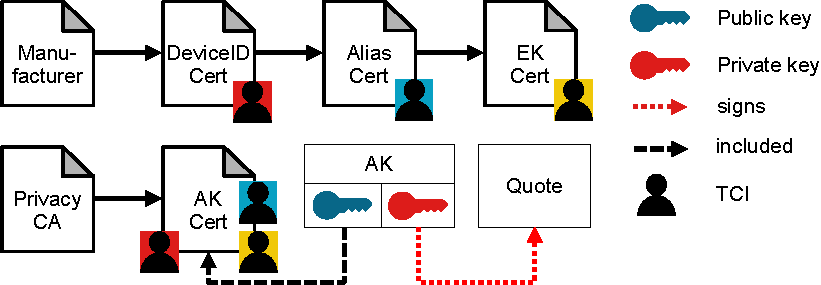
\includegraphics[width=1\linewidth]{figures/privacy-arch.pdf}
  \caption{The adapted architecture integrating privacy.} \label{fig:privacy_arch}
\end{figure}


% General: Contradiction
% Goal of DICE is explicitly to establish a long-term identity. So, we need to work against its design.

% Maybe: The certificates would need to be encrypted as well, as they contain the TCI values, potentially identifying the device

% Use Attestation key not in endorsement (and platform?) hierarchy

% Each AliasKey is a identity key as specified in DICE layering Architecture 8.1.1.5
% They would need to be made independent of the devices identity.

% TODO: Maybe put somewhere earlier
% In general, endorsement keys represent device identities and are therefore privacy-sensitive.
% Our EK takes on the role of an attestation key, which has the task of signing attestation evidences.
% Although our EK does not represent the device identity, it does represent the identity of the shorter lived fTPM.
% This makes our EK also privacy-sensitive, since its generated signatures can be cross-referenced and then traced back to the according EK.
% Our approach has the advantage that we do not need a trusted third party, but trust the manufacturer of our trust anchor directly (DICE).
% In \autoref{sec:privacy}, an extension of our system is presented with privacy in mind.
